\chapter{Атака оптической накачкой на источник когерентного излучения}\label{ch:ch4}
\renewcommand{\thefigure}{4.\arabic{figure}} % Plain numbering
\setcounter{figure}{0}                     % Reset if needed


Использование технологии квантового распределения ключей дает абсолютную защиту информации от доступа злоумышленника за счет использования метода одноразовых блокнотов для шифрования данных и за счет использования одиночных фотонов в качестве носителей ключа для его передачи через оптические линии связи, применение которых обеспечивает безопасность за счет фундаментальных законов квантовой физики \cite{bennett1984,horodecki2008}. Однако несовершенство технических компонентов, применяемых в практических реализациях систем КРК, может дать злоумышленнику доступ к секретному ключу за счет внесения изменений в функционирование элементов или, что хуже, полностью контролировать их работу \cite{lo2014,dixon2017,xu2020,makarov2023}. Поэтому критически необходимо исследовать потенциальное влияние злоумышленника на элементы в составе систем квантового распределения ключа. В данной главе рассматривается новый тип атаки на источник когерентного излучения - атака оптической накачкой.

\section{Атака оптической накачкой на лазер с распределенной обратной связью}\label{sec:ch4/sec1}
Существующие источники когерентного излучения в системах квантового распределения ключа могут подвергаться воздействию злоумышленника по изменению его характеристик. На это нацелена атака лазерным засеиванием. Суть которого заключается в том, что Злоумышленник (Ева) вводит свое излучение в резонатор лазера с распределенной обратной связью, используемый Алисой для передачи квантовых состояний. В результате этого воздействия, изменяется выходная мощность излучения, форма и площадь импульса \cite{huang2019, pang2020}. При этом воздействие возможно даже изменение длины волны. Эти эффекты могут быть использованы Евой для получения информации о ключе.
Данная атака задействует механизм оптической инжекции, рассмотренный ранее, используя длину волны лазера, близкую к рабочей длине волны лазера Алисы.
\newline Однако существующие уязвимости в пассивных оптических компонентах \cite{nasedkin2022, nasedkin2023,borisova2020}, используемых для защиты от других типов атак, позволяют Еве использовать другие длины волн для проведения своих манипуляций по изменению характеристик излучения \cite{lovic2023}. Для этих целей может быть использовано излучение на длине волны 1310 нм. Данная глава посвящена проведению атаки оптической накачкой \cite{svelto1998, okamoto2003,klinkhammer2012, guina2017} на полупроводниковый лазер с распределенной обратной связью, работающим в режиме переключения усиления \cite{svelto2010}. Измерялись параметры выходного излучения, его мощность, ватт-амперная характеристика. Изучается влияние оптической накачки на длине волны 1310 нм на форму и площадь импульсов. 
Схема эксперимента представлена на \ref{fig:ch4 1310 exp}.
\begin{figure}
    \centering
    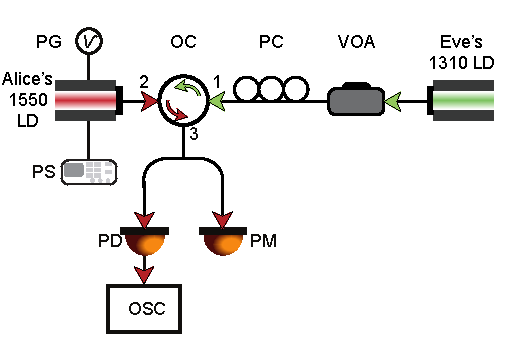
\includegraphics{images/1310 experiment (3).pdf}
    \caption{Экспериментальная установка по проведению атаки оптической накачкой на источник когерентного излучения из состава системы квантового распределения ключей. Alice's LD - лазерный диод Алисы, PG - генератор импульсов, PS - источник напряжения, OC - оптический циркулятор, PC - контроллер поляризации, VOA - перестраиваемый оптический аттенюатор, Eve's LD - лазер Евы, PM - измеритель мощности, PD - фотодиод, Osc - осциллограф.}
    \label{fig:ch4 1310 exp}
\end{figure}
Данная схема работает следующим образом. На лазер Алисы (LD1550, Agilecom WSLS-934010C4124-82) подается ток смещения с помощью лабораторного блока питания. Величина тока накачки должна не превышать порогового значения. После этого подаются импульсы с генератора импульсов для работы лазерного диода в режиме переключения генерации. Выход лазерного диода подключен ко 2 выходу оптического циркулятора с сохранением поляризации. В первый же вход циркулятора подается излучение от лазера Евы. Ее лазер также основан на полупроводниковом кристалле с распределенной обратной связью, однако его рабочая длина волны составляет 1310 нм, когда лазер Алисы работает на длине волны 1550 нм. Непрерывное излучение от лазера Евы попадает на переменный оптический аттенюатор (OZ Optics, BB-100) для изменения выходной мощности лазера без изменения тока накачки, увеличение или уменьшение которого приводит к изменению длины волны лазера, что является критичным изменением для воспроизводимости эксперимента. После этого излучения попадает на механический контроллер поляризации для согласования оси поляризации выходного излучения с осью поляризации оптического циркулятора и лазера соответственно для максимальной эффективности ввода оптического излучения в резонатор лазера Алисы. Попадая на 1 вход оптического циркулятора, излучение Евы проходит его без изменений и с небольшим затуханием попадает в волоконный вывод лазера Алисы. Распространяясь по нему, оно попадает на зеркало кристалла, от которого оно частично отражается, а частично проходит внутрь. Для очистки данных была измерена мощность излучения, отраженного от всех элементов лазера и вычтена из полученных результатов. В результате прошедшее излучение поглощается кристаллом InGaAs и благодаря этому создается дополнительная инверсия населенностей в кристалле, которая повышает выходную мощность лазерного излучения на длине волны 1550 нм. Влияние этого эффекта и рассматривается в данной главе. 
%\section{Изменение Ватт-Амперной характеристики лазера с распределенной обратной связью при атаке на рабочей длине волны}\label{sec:ch4/sect2}

\section{Изменение Ватт-Амперной характеристики лазера с распределенной обратной связью при атаке на других длинах волн}\label{sec:ch4/sect3}
Одной из основных характеристик лазера является его ватт-амперная характеристика. Эта кривая показывает зависимость прироста мощности выходного излучения в зависимости от тока накачки, пропускаемого через кристалл. В рамках данного раздела описывается изменение этой характеристики в зависимости от мощности лазера Евы.
Для этого лазер Алисы работал в непрерывном режиме только с накачкой током от лабораторного блока питания. Мощность контролировалась оптическим измерителем мощности (Thorlabs, PM400). А ток накачки лазера варьировался от 0 до 25 мА. 
Результат измерения данных характеристик представлен на рисунке \ref{fig:Watt-Amp ch4}.
\begin{figure}
    \centering
    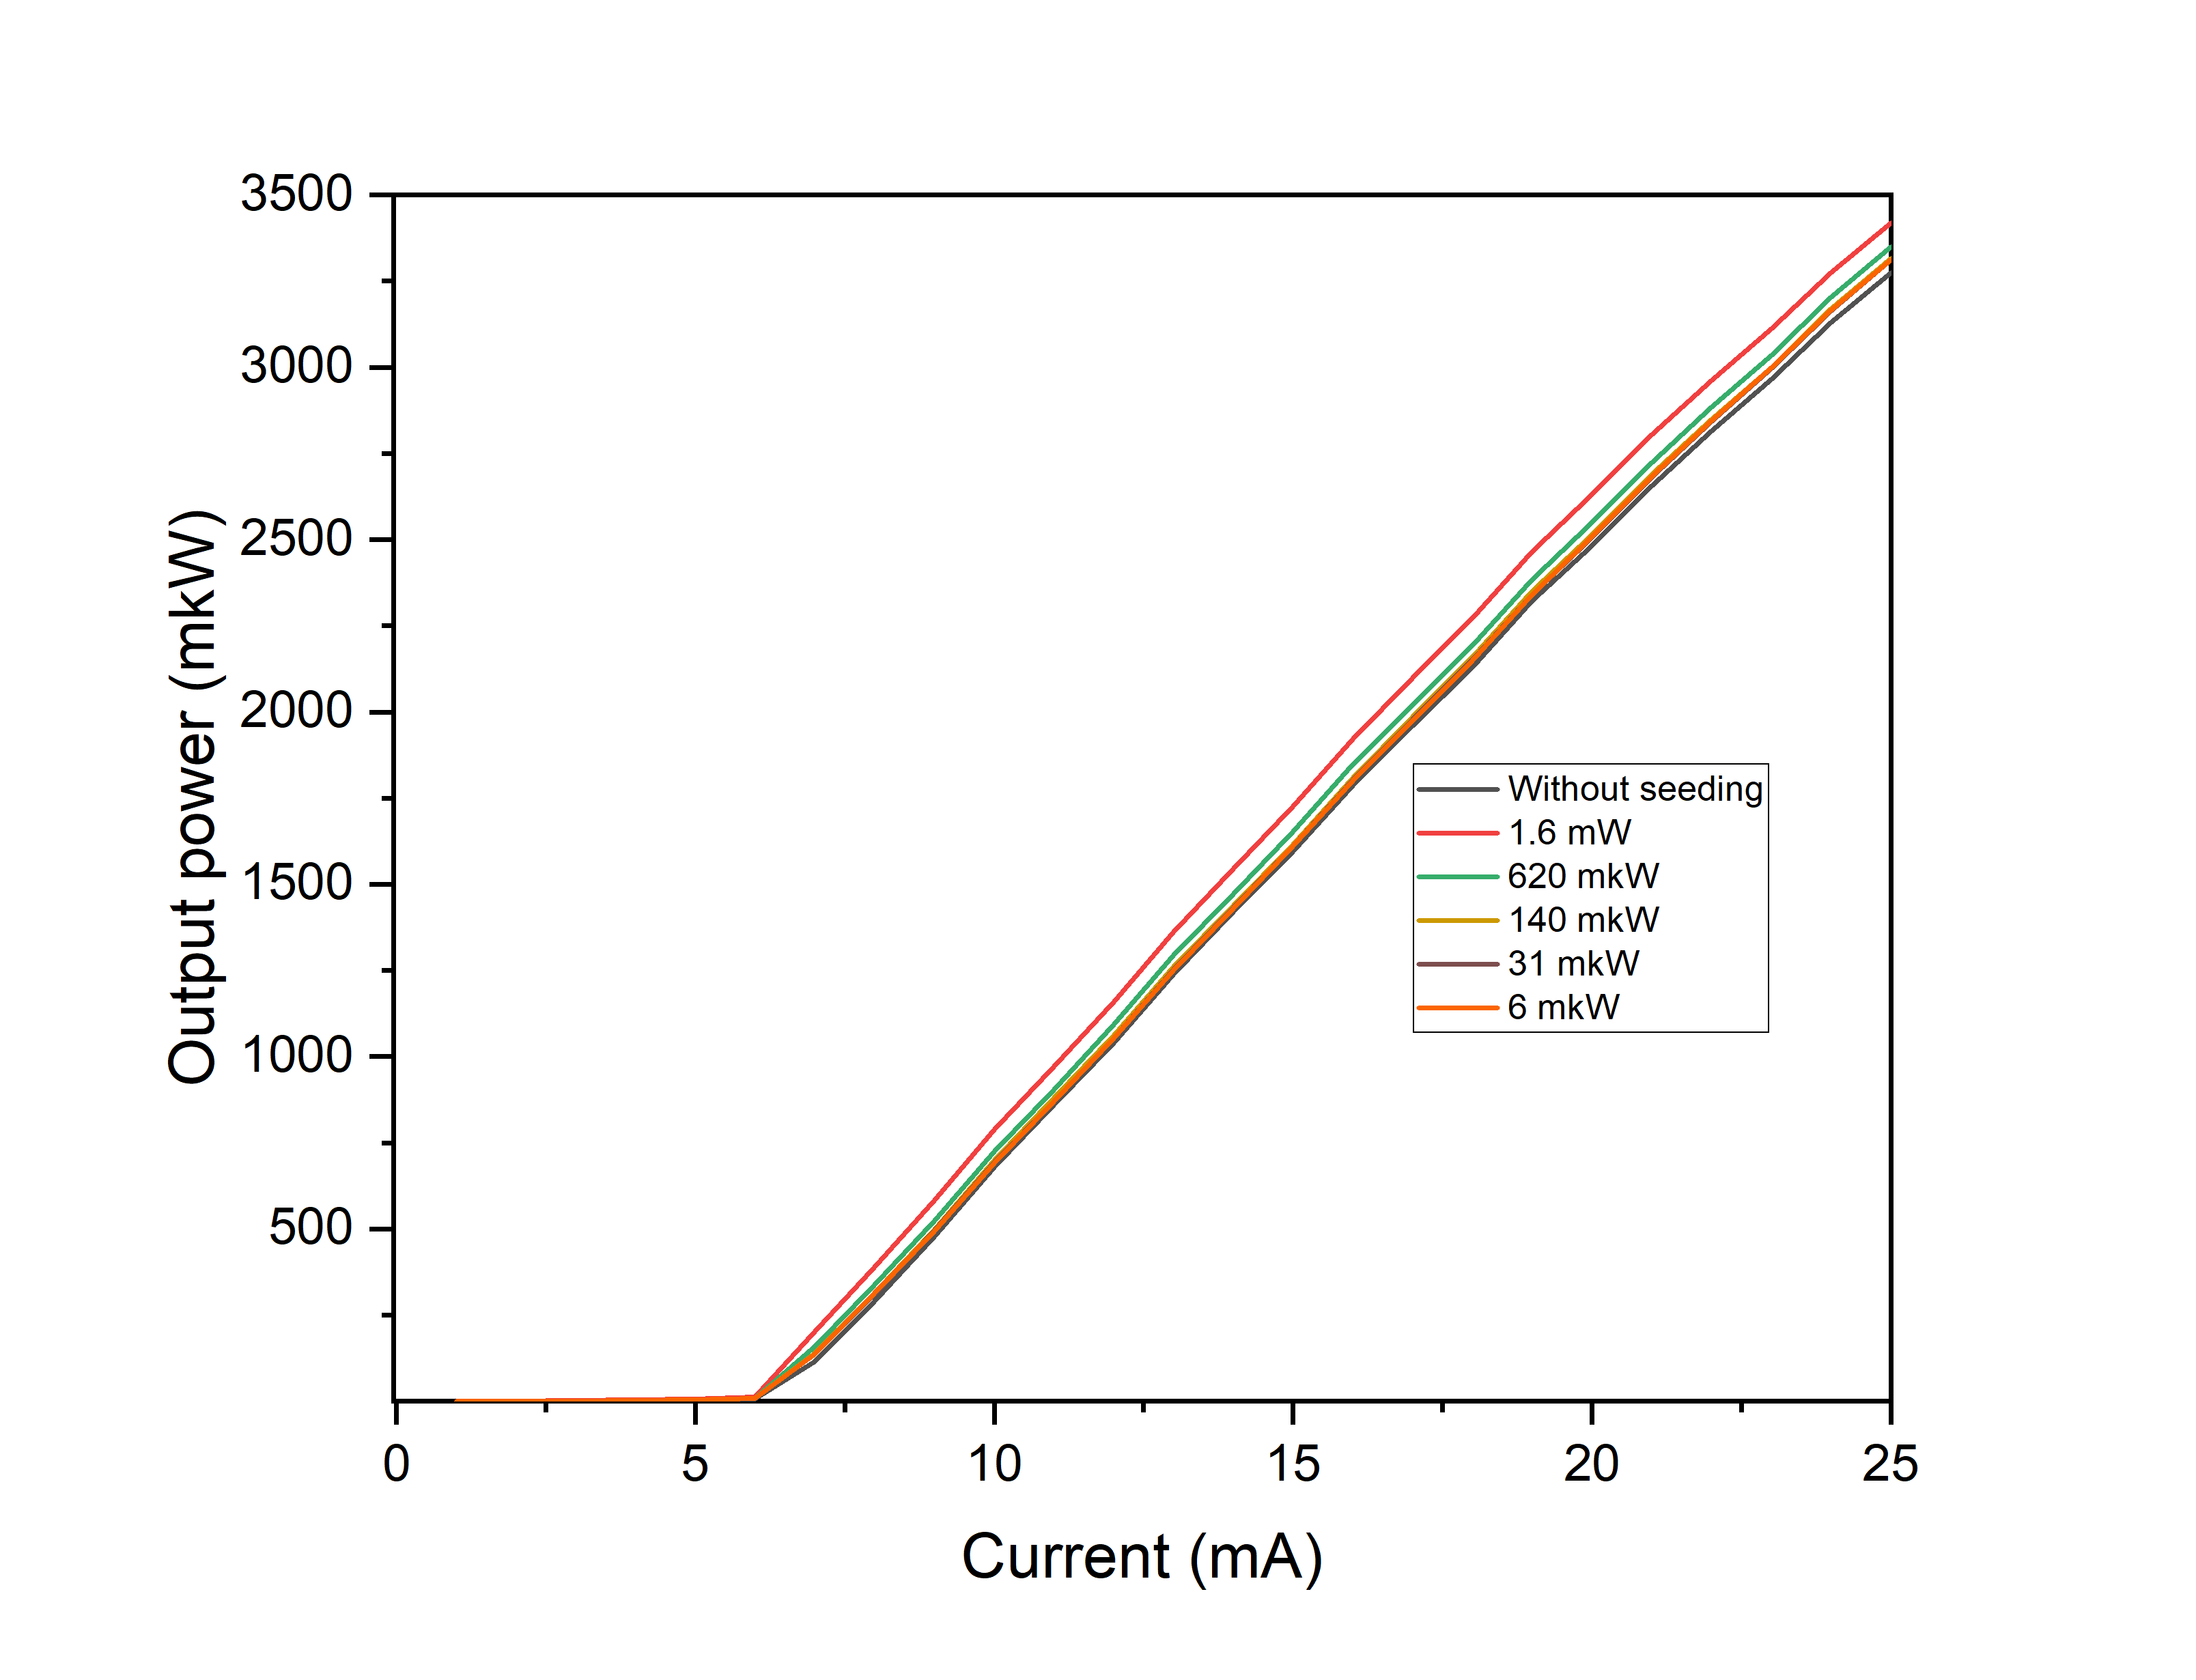
\includegraphics[width=\linewidth]{images/ватт ампер для диссера.png}
    \caption{Ватт-Амперные характеристики лазера Алисы под действием внешней оптической накачки от Евы.}
    \label{fig:Watt-Amp ch4}
\end{figure}
Данные графики демонстрируют, что дополнительная накачка от Евы в диапазоне мощностей от 1.6 мВт до 31 мкВт сдвигает исходную Ватт-Амперную кривую, что показывает возможность Евы манипулировать мощностью Алисы. Для численной оценки этого влияния необходимо перейти к дифференциальной квантовой эффективности \cite{cassidy1984,tomiyasu2017}. Эта величина показывает эффективность преобразования электронного тока в фотоны, излучаемые лазером. Формула расчета величины дифференциальной квантовой эффективности ниже 
\begin{equation}
\eta = \frac{2e}{\hbar\omega}\frac{dP}{dI}
\label{eq:quaneff}
\end{equation}, 
где $\eta$ - дифференциальная квантовая эффективность, e - заряд электрона, $\hbar$ - приведенная постоянная Планка, $\omega$ - частота лазера, $dP/dI$ - аппроксимированное значение производной измеренных Ватт-Амперных характеристик.
В результате этих вычислений показано на рисунке \ref{fig:diff quant eff ch4}, что Ева, используя оптическую накачку на 1310 нм, изменяет дифференциальную квантовую эффективность лазера Алисы, что приводит к увеличению выходной мощности лазера при неизменном токе накачки.
\begin{figure}
    \centering
    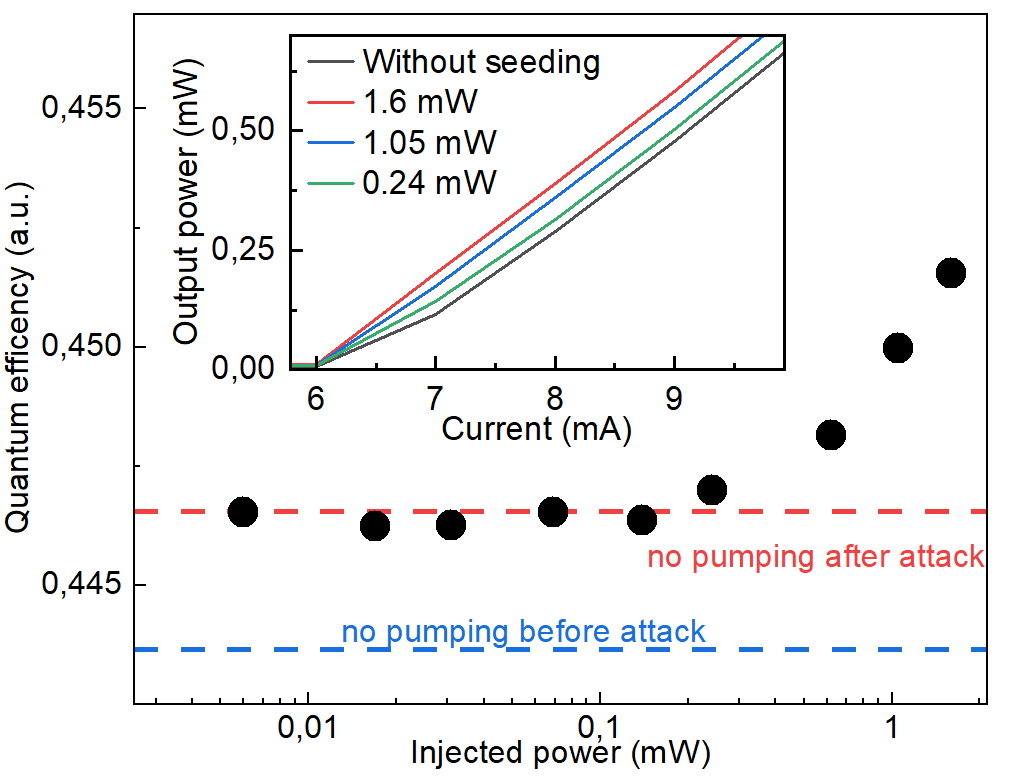
\includegraphics{images/Эффективность 1310.png}
    \caption{График зависимости дифференциальной квантовой эффективности в зависимости от мощности накачки Евы. Красная пунктирная линия обозначает значение дифференциальной квантовой эффективности после проведенной атаки, а синяя пунктирная линия обозначает значение дифференциальной квантовой эффективности до атаки.}
    \label{fig:diff quant eff ch4}
\end{figure}
В результате аппроксимации наклона ватт-амперных характеристик и расчета дифференциальной квантовой эффективности (ДКЭ) по формуле \ref{eq:quaneff} было показано, что Ева может увеличивать ДКЭ на несколько процентов, что негативно сказывается на скорости выработки секретного ключа и этот эффект должен быть учтен. 

\section{Изменение формы импульса при атаке на лазер с распределенной обратной связью, работающем в режиме переключения усиления}\label{sec:ch4/sect4} 
Для измерения влияния оптической накачки на форму и энергию импульсов, сгенерированных Алисой, необходимо использовать лазер Алисы в импульсном режиме. Для этого атакуемый лазер был переведен в режим работы переключения усиления для генерации импульсов. Ток накачки составил 3 мА. Импульсы же генерировались генератором импульсов (P400, Highland Technology). Полученные импульсы регистрировались опто-электронным конвертором (PDI35-10G, Laserscom) и оцифровывалось осциллографом 735Zi, Lecroy, с полосой пропускания 3.5 GHz, скорость оцифровки 40 GS/s. Для синхронизации на осциллограф был дополнительно выведен электрический сигнал с генератора импульсов для запуска развертки и точного измерения времени прихода импульсов. Частота повторения этих импульсов составляла 10 MHz и длительность импульса составляла 700 ps. Результат измерения этих импульсов представлен на рисунке \ref{fig:pulse shape ch4}.
\begin{figure}
    \centering
    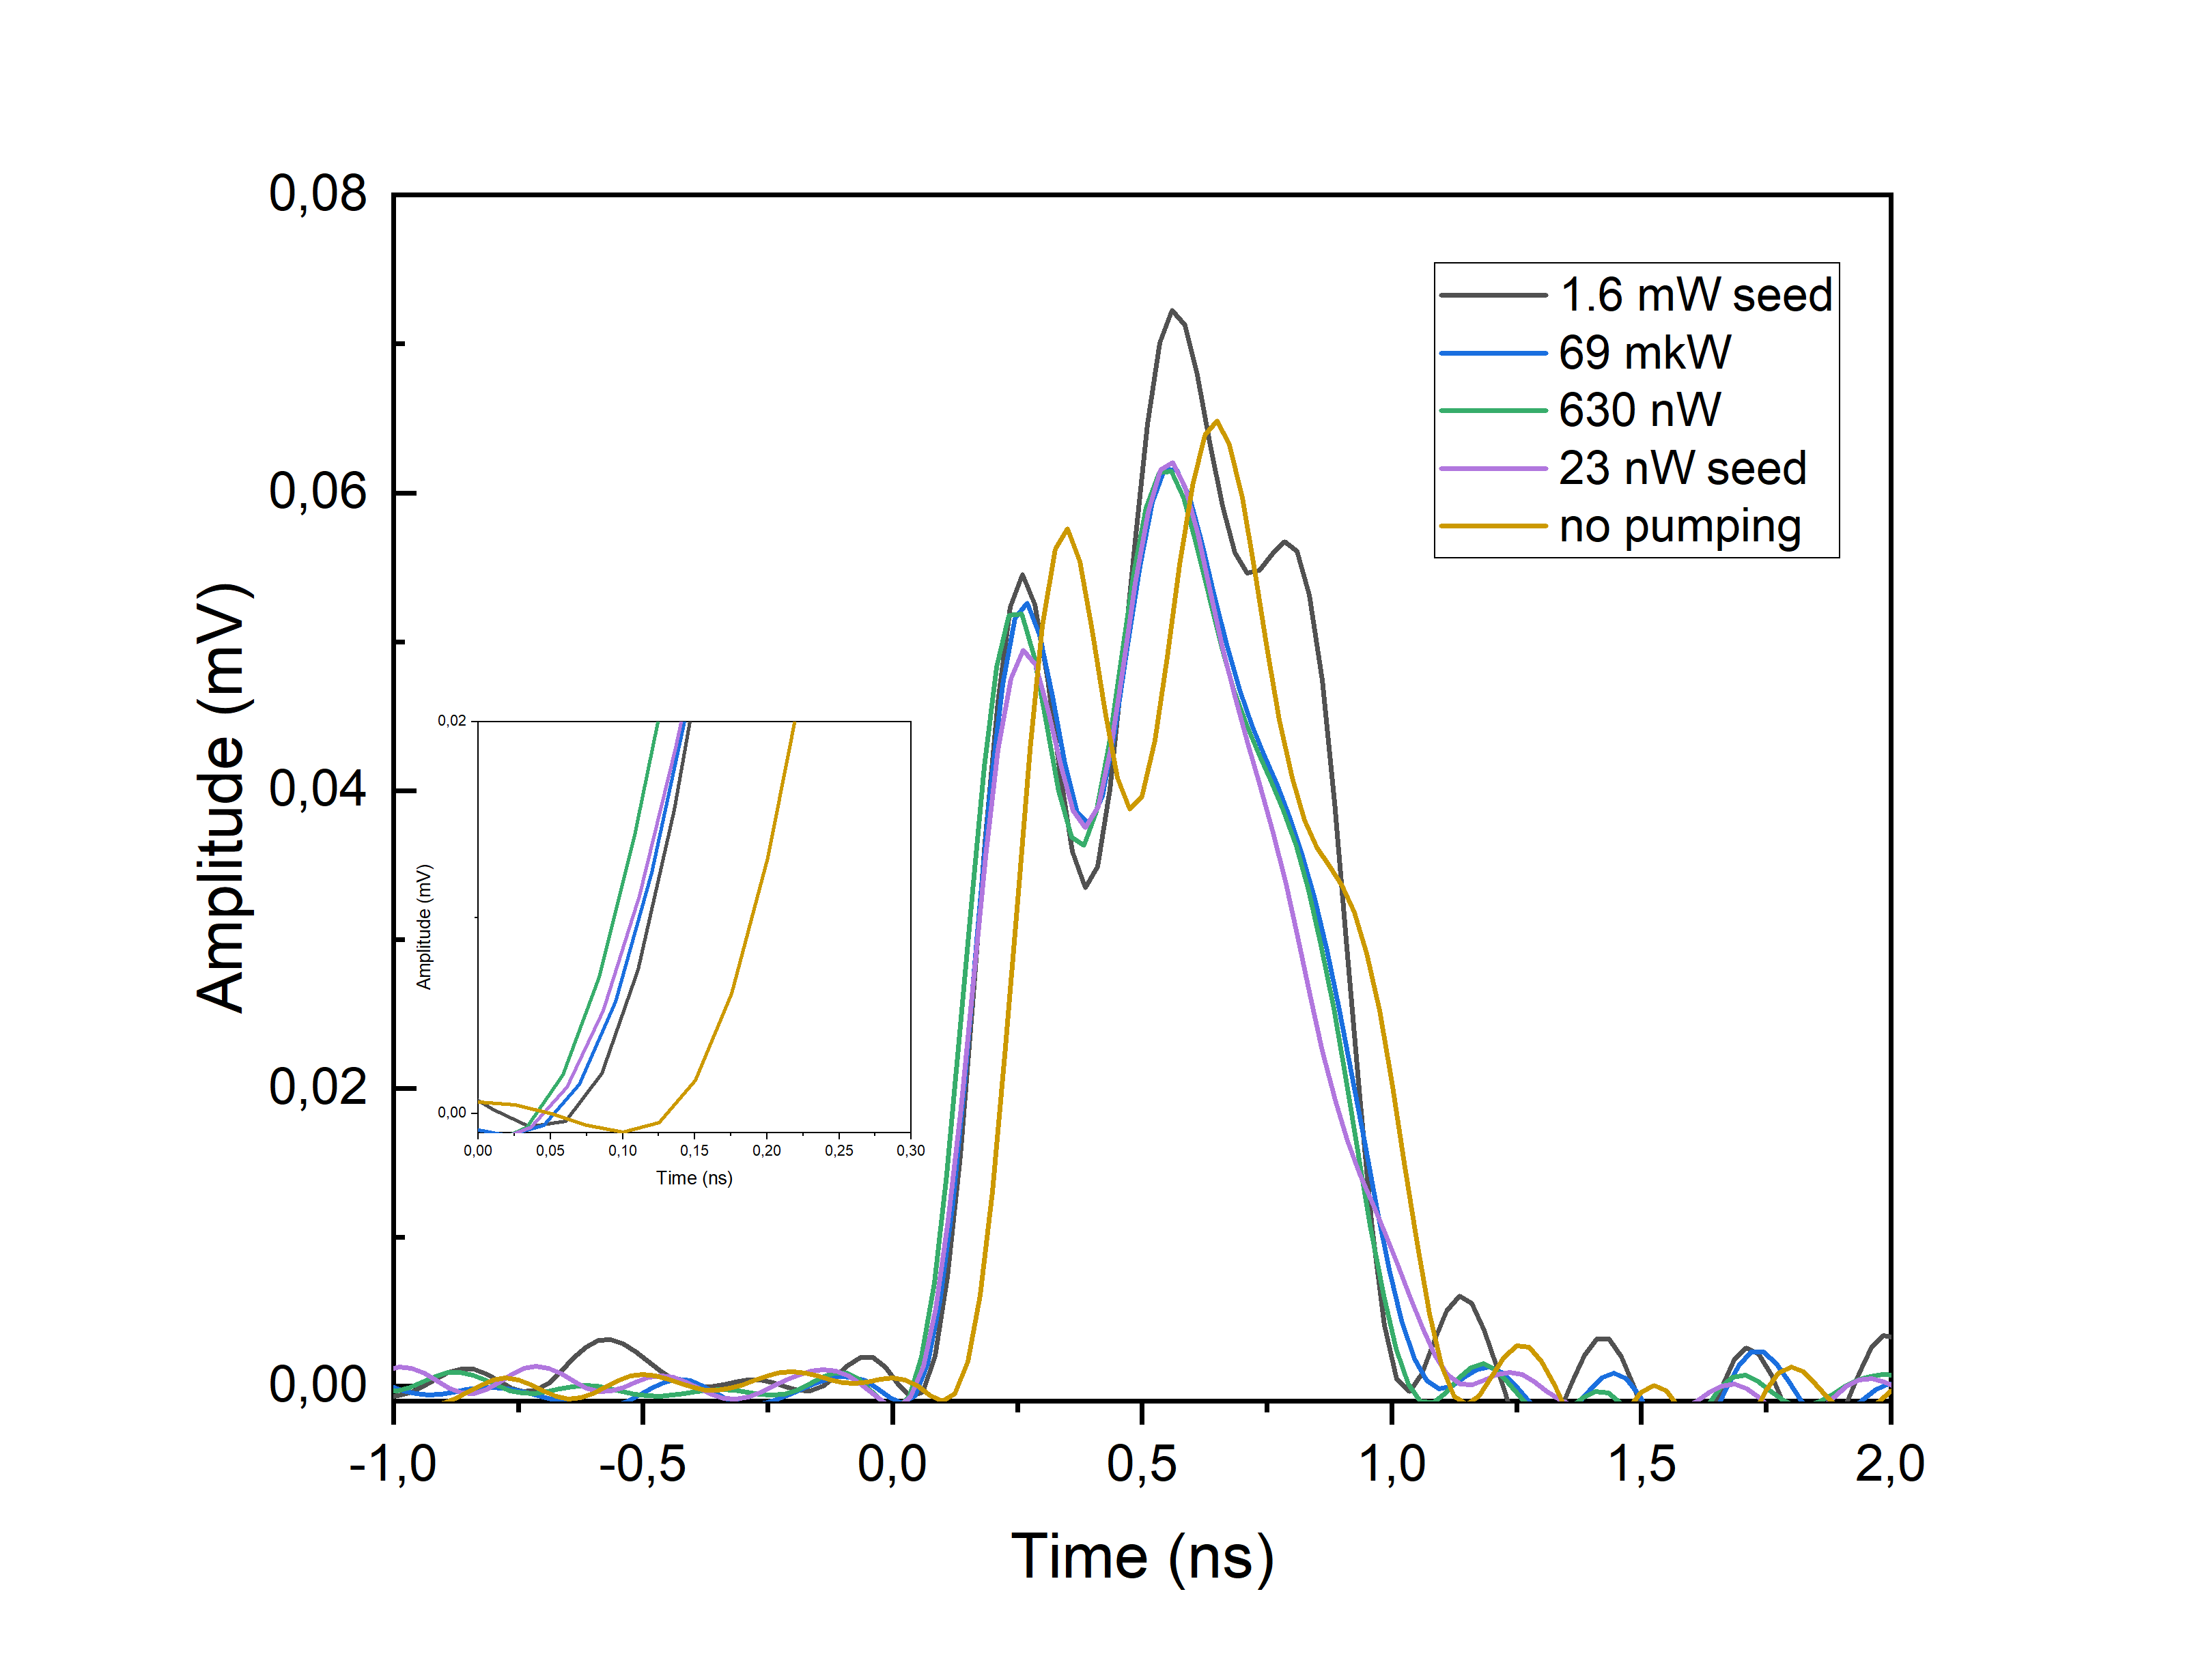
\includegraphics[width=\linewidth]{images/Импульсы под действием 1310 для диссера.png}
    \caption{Формы импульсов, сгенерированных Алисой, под действием оптической накачки и без нее.}
    \label{fig:pulse shape ch4}
\end{figure}
Как видно из рисунка \ref{fig:pulse shape ch4}, дополнительная накачка Евы не только увеличивает выходную энергию импульсов, а также сдвигает их время генерации на величину приблизительно равной 100 пс. Для оценки влияния оптической накачки на площадь импульсов, исследуемые импульсы были оцифрованы и их площадь была проинтегрирована в программной среде Origin. Результаты этого интегрирования представлены на рисунке \ref{fig:energy 1310 ch4}.
\begin{figure}
    \centering
    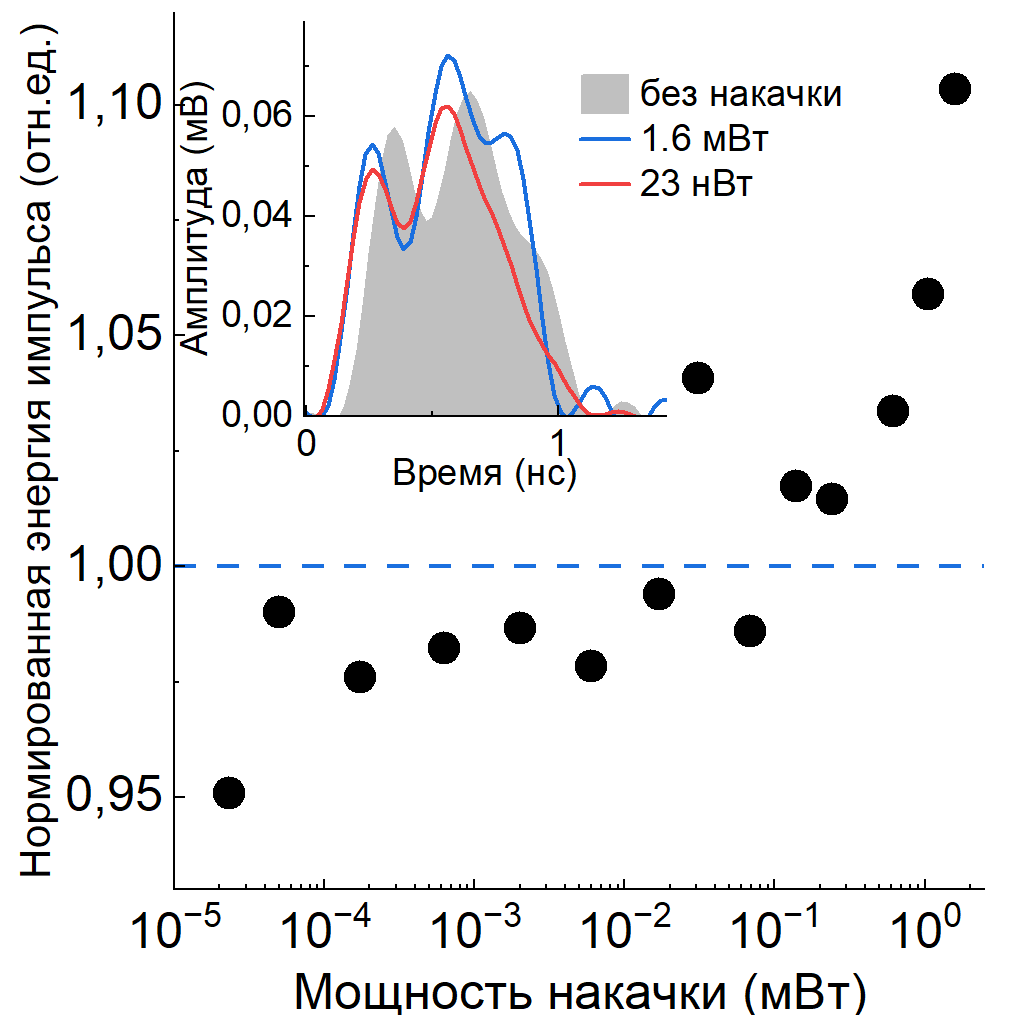
\includegraphics[width=\linewidth]{images/1310_энергия.png}
    \caption{Изменение энергии импульсов под действием накачки лазером на длине волны 1310 нм Евы.}
    \label{fig:energy 1310 ch4}
\end{figure}
Проведенные измерения показывают, что воздействие Евы изменяет не только дифференциальную квантовую эффективность, но и энергию импульсов, излучаемой Алисой, что позволяет также снижать дальность и скорость выработки секретного ключа. В результате воздействия энергия импульсов не только может увеличиться на 10 процентов, но даже может уменьшится при некоторых мощностях оптического излучения накачки.
\newline Для полной картины изменения мощности, излучаемой Алисой под действием оптической накачки злоумышленника, необходимо оценить еще и средний уровень мощности. Для этого используется лазер, работающий в импульсном режиме, как и описано выше, однако мощность измеряется с помощью измерителя оптической мощности (ИОМ). Скорость работы данного ИОМ не позволяет измерить мощность каждого импульса, поэтому он интегрирует всю мощность и импульсную, и непрерывную. Результат измерения показан на рисунке \ref{fig:avg pwr 1310 ch4} 
\begin{figure}
    \centering
    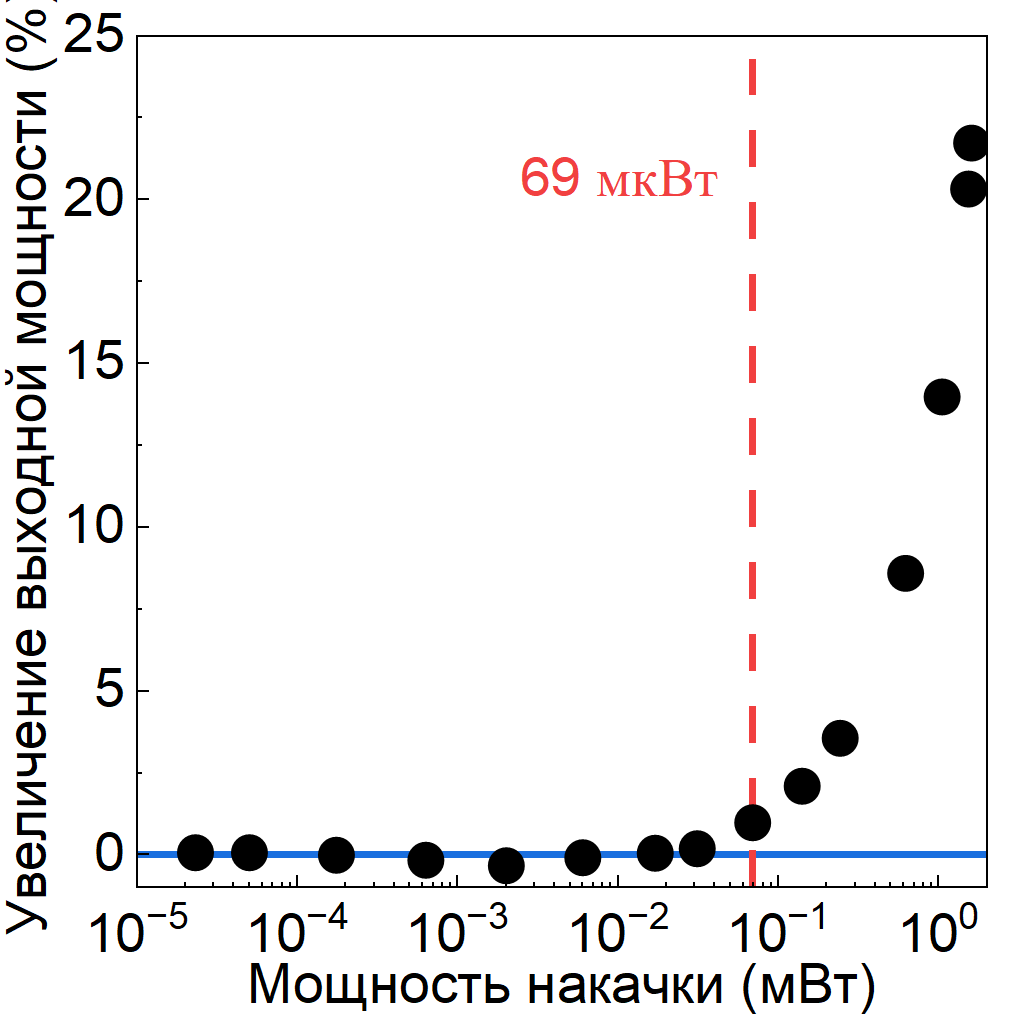
\includegraphics{images/1310_мощность.png}
    \caption{Изменение средней мощности лазера Алисы под действием оптической накачки Евы.}
    \label{fig:avg pwr 1310 ch4}
\end{figure}
В результате воздействия Евы, мощность лазера с распределенной обратной связью увеличивается на 20\%, когда как значение энергии импульсов повышается только на 10\%. Что объясняется тем, что Ева также повышает и непрерывное излучение из лазера Алисы.
\section{Определение минимально необходимой изоляции лазерного источника для предотвращения атаки оптической накачкой}\label{sec:ch4/sect5}
В качестве исходной мощности, которая необходима для создания заметного эффекта, определенная ранее в этом разделе составляет 70 мкВт или -11.6 дБм. Существующие на рынке решения предлагают лазеры, способные выдавать 14 Вт или 41.46 дБм мощности на длине волны 1310 нм \cite{grimes2022}.
Для определения изоляции необходимо вычесть из мощности лазера минимально необходимую мощность для создания эффекта по формуле \ref{eq:1310_iso}.
\begin{equation}
\label{eq:1310_iso}
    \alpha_{iso} = P_{laser} - P_{req}
\end{equation}
В результате вычислений величина изоляции, необходимая для предотвращения атаки оптической накачкой составляет 53 дБ. 

\section{Оценка возможности проведения атаки на существующие системы квантового распределения ключей}\label{sec:ch4/sect6}
Современные системы квантового распределения ключей содержат в себе элементы, предназначенные для защиты от различных атак на техническую реализацию. К таким элементам относятся различные пассивные фильтры и изоляторы.
Однако некоторые защитные элементы могут вести себя непредсказуемо для разных длин волн. Эти особенности позволяют злоумышленнику их использовать для получения информации о ключе.
Ярким примером могут служить DWDM (Dense Wavelength Division Multiplexion) фильтры и оптические изоляторы. Их заявленные характеристики соблюдаются только в относительно небольшом диапазоне длин волн.
С изменением зондирующей длиной волны изменяется и величина изоляции, вносимой элементом. Пример этого эффекта отображен на рисунке \ref{fig:isolation_spectrums}
\begin{figure}
    \centering
    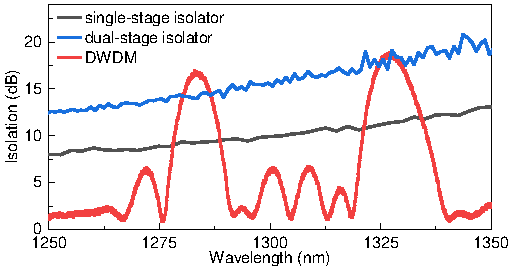
\includegraphics[width=\linewidth]{spectra_1310_iso.pdf}
    \caption{Величина изоляции пассивных элементов, используемых в системах КРК. Красным цветом обозначен спектр изоляции DWDM фильтра, серым - одностадийного изолятора, синим - двухстадийного изолятора}
    \label{fig:isolation_spectrums}
\end{figure}
Как видно из рисунка \ref{fig:isolation_spectrums}, представленные элементы не вносят существенной изоляции как на рабочей длине волны. К примеру, изоляция одностадийного изолятора на длине волны 1550 нм составляет 30 дБ, а двухстадийного - 40 дБ. Однако на длине волне 1310 нм эти величины составляют 8 и 12.5 дБ соответственно.
Когда DWDM фильтр на длине волны 1310 нм вносит 5 дБ, в то время как на длине волны 1550 нм вносит 30 дБ потерь \cite{ponosova2022}. Таким образом видно, что пассивные элементы не вносят заявленной изоляции и эта лазейка может быть использован злоумышленником.
В качестве схемы КРК будет использоваться схема из работы \cite{makarov2023}. 
\begin{figure}
    \centering
    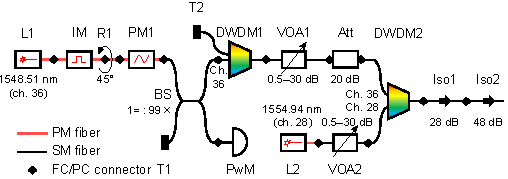
\includegraphics[width=\linewidth]{Qrate-Alice.pdf}
    \caption{Оптическая схема блока Алиса}\label{fig:Alice_qrate}
\end{figure}
Для расчета необходимой минимальной зондирующей мощности необходимо просуммировать все потери, вносимые элементами на длине волны 1310 нм. 
Измеренные значения потерь элементов продемонстрировано в таблице \ref{tab:isolation1310}

\begin{tabular}[t]{lll}
    \hline\hline
    Элемент & Потери, дБ  \\
    \hline
    Встроенный изолятор в лазере &10.5 \\
    Изолятор 1  & 10.56 &  \\
    Изолятор  2 & 16.24 &  \\
    Фиксированный аттенюатор & 19.6  \\
    Переменный аттенюатор & 0.5 \\
    Светоделитель & 23.98 \\
    DWDM1  & 4.08  \\
    DWDM2  & 3.03  \\
    Фазовый модулятор & 4.5  \\
    Модулятор интенсивности & 4.5 \\
    \hline\hline
    \end{tabular}
      \label{tab:isolation1310}
%\end{table}

Вычисления производятся по формуле 
\begin{equation}
    \begin{split}
    \alpha_{1310}=\alpha_\text{Iso1} + \alpha_\text{Iso2} + \alpha_\text{Att} + \alpha_\text{VOA1} + 2\alpha_\text{DWDM} +\\
     \alpha_\text{PM} + \alpha_\text{IM} + \alpha_\text{LD},
     \end{split}
    \label{eq:input power}
\end{equation}
где $\alpha_{Iso}$ вносимые потери изолятором на длине волны 1310 нанометров, $\alpha_{att}$, $\alpha_{VOA}$ , $\alpha_{DWMD}$, $\alpha_{PM}$, $\alpha_{IM}$, и $\alpha_{LD}$ вносимые потери компонентов \ref{fig:Alice_qrate}.
Для определения потерь использовались схожие компоненты как в работе \cite{makarov2023}. Раскрывать модели всех элементов не представляется возможным по соображениям конфиденциальности. 
Но эти элементы представляют собой стандартные телекоммуникационные элементы доступные для заказа. Потери на длине волны 1310 нм фиксированного аттенюатора (Thorlabs FA20T) и светоделителя 99:1 (Thorlabs TW1550R1A2) определены в даташите производителем.
Потери фазового модулятора на основе кристалла Ниобата Лития, легированного Титаном, измерялись с помощью лазера, который используется в эксперименте, и измерителем мощности. Потери в модуляторе интенсивности считаем аналогичными.
Остальные же элементы измерялись с помощью источника суперконтиниума и оптического анализатора спектра (HP Hewlett Packard 70004A) по методологии, описанной в \cite{makarov2023}. Потери на изоляторе, встроенном в лазерный диод, считаем аналогичными одностадийному изолятору в 10 дБ.
В итоге изоляция всей системы, изображенной на \cref{fig:Alice_qrate} составляет 97.55 дБ, что существенно превышает минимальное определенное значение в 53 дБ. Поэтому данная система устойчива к атаке оптической накачкой. 


\section{Выводы по главе}\label{sec:ch4/sect7}
В данной главе рассматривается новый тип атаки на источники лазерного излучения - атака оптической накачкой, на примере накачки на длине волны 1310 нм. Однако, данный эффект наблюдается в широком диапазоне длин волн, обусловленном шириной полосы поглощения полупроводникового кристалла, на котором построен DFB лазер. 
Изучено влияние на интенсивность излучаемой мощности, определена минимально необходимая мощность для создания заметного эффекта в 70 мкВт. Определена минимально необходимая изоляция для предотвращения атаки оптической накачкой на длине волны 1310 нм и зондирующей мощностью 500 мВт в 53 дБ.
Определена стойкость существующей системы квантового распределения ключей к атаке оптической накачкой. Ее суммарная изоляция составила 97.55 дБ, что превышает минимальное пороговое значение в 53 дБ, что делает данную систему устойчивой к атаке оптической накачкой. 
